\documentclass[a4paper,14pt]{extarticle} % 14й шрифт
\usepackage{extsizes}
\usepackage{cmap} % для кодировки шрифтов в pdf
\usepackage[T2A]{fontenc}
\usepackage[utf8]{inputenc}
\usepackage[russian]{babel}
\usepackage{amssymb,amsfonts,amsmath,amsthm} % математические дополнения от АМС
\usepackage[left=20mm, top=15mm, right=15mm, bottom=15mm, nohead, footskip=10mm]{geometry} % настройки полей документа
\usepackage{graphicx}
\usepackage{float}
\usepackage{textcomp}
\usepackage{subcaption}
\usepackage{amsthm}% настройки полей документа

\renewcommand{\rmdefault}{ftm} % Times New Roman
\frenchspacing

\newtheorem{definition}{Определение}
\newtheorem{theorem}{Теорема}
 
\begin{document} % начало документа


 
% НАЧАЛО ТИТУЛЬНОГО ЛИСТА
\begin{center}
\hfill \break
\normalsize{Санкт-Петербургский государственный университет}\\ 
\hfill \break
\normalsize{Отделение прикладной математики и информатики}\\
\normalsize{\textbf{Кафедра прикладной кибернетики}}\\
\hfill \break
\hfill \break 
\hfill \break
\hfill \break
\hfill\break
\hfill \break
\normalsize{Миронов Алексей Владиславович}\\
\hfill \break
\large{Оценка области захвата для систем ФАПЧ 3 порядка}\\
\hfill \break
\small{Выпускная квалификационная работа}\\
\hfill \break
\hfill \break
\hfill \break
\hfill \break
\hfill \break
\hfill \break
\hfill \break
\hfill \break
\end{center}
 
\hfill \break
\hfill \break
\hfill \break
 
 \small{
\begin{flushright}
Научный руководитель:\\
д. т.н., профессор Юлдашев Р. В.
\end{flushright}
}
\hfill \break
\hfill \break
\hfill \break
\hfill \break
\hfill \break
\hfill \break
\hfill \break
\hfill \break
\hfill \break
\hfill \break
\hfill \break
\hfill \break
\hfill \break
\begin{center} Санкт-Петербург \\
2019 \end{center}
\thispagestyle{empty} % выключаем отображение номера для этой страницы
% КОНЕЦ ТИТУЛЬНОГО ЛИСТА

 \tableofcontents
\newpage
\section{Введение}
Рассмотрим систему:
 \begin{equation}\label{etalon_system}
 \begin{aligned}
 &\dot{x} = Ax + b\upsilon_e(\theta_e)\\
 &\dot{\theta_e} = \omega_e^{free} - K_{vco}(c^*x + h\upsilon_e(\theta_e))
 \end{aligned}
\end{equation}
Найдем стационарные точки системы \eqref{etalon_system}
 \begin{equation}\label{transition}
 \begin{aligned}
 &x = -A^{-1}b\upsilon_e(\theta_e)\\
 &\upsilon_e(\theta_e) = \frac{\omega_e^{free}}{K_{vco}H(0)}
 \end{aligned}
\end{equation}
Возьмем $\theta_e = \theta_s$, для которых выполняется \eqref{transition}. Сделаем замену:
 \begin{equation}\label{replacement1}
 \begin{aligned}
 &z =x + A^{-1}b\upsilon_e(\theta_s)\\
 &\sigma = \theta_e 
 \end{aligned}
\end{equation}
После замены система \eqref{etalon_system} принимает вид:
 \begin{equation}
 \begin{aligned}
 &\dot{z} = Az + b(\upsilon_e(\sigma) - \frac{\omega_e^{free}}{K_{vco}H(0)})\\
 &\dot{\sigma} = -K_{vco}(c^*z + h(\upsilon_e(\sigma) - \frac{\omega_e^{free}}{K_{vco}H(0)}))
 \end{aligned}
\end{equation}

\section{Теорема}
Рассмотрим систему:
 \begin{equation}\label{system}
 \begin{aligned}
 &\dot{z} = Az + Bf(\sigma)\\
 &\dot{\sigma} = C^*z + Rf(\sigma)
 \end{aligned}
\end{equation}

Here A, B, C, and R are constant matrices of dimensions n × n, n × m, n × m, and n × n, respectively, whereas the components $\phi_k$, $1 \leq  k \leq m$, of the vector-valued function $f(\sigma)$ are scalar differen-tiable functions $\phi_k$ = $\phi_k(\sigma_k)$, where $\psi_k$ is the k-th component of the vector $\psi$.\\

Recall that any pendulum-like system with a single scalar non-linearity and an irreducible transfer function $\chi(p)$ can be written in the form \eqref{system} with m = 1 by a nonsingular linear transformation of phase coordinates. Further we assume that the functions $\phi_k(\sigma_k)$ satisfy the followingconditions: $\phi_k(\sigma_k) \equiv 0$\\
 \begin{equation}
 \begin{aligned}
&\mu_{1k} \leq \frac{d\varphi_k(\sigma_k)}{d\sigma_k} \leq \mu_{2k}, \forall \sigma_k \in \mathbb{R}\\
&\varphi_k(\sigma_k+\Delta_k) = \varphi_k(\sigma_k), \forall \sigma_k \in \mathbb{R}
 \end{aligned}
\end{equation}
Here the $\Delta_k$ are positive numbers. Sometimes, in the study of the specific pendulum-like systems, only one of the inequalities
 \begin{equation}
 \begin{aligned}
\mu_{1k} \leq \frac{d\varphi_k(\sigma_k)}{d\sigma_k}  or \frac{d\varphi_k(\sigma_k)}{d\sigma_k} \leq \mu_{2k}
 \end{aligned}
\end{equation}
is known, so we will assume the number $mu_{1k}$ to be either finite negative or $-\inf$, and the number $\mu_{2k}$ to be either finite positive or $\inf$.
When $\mu_{1k} = -\inf$ or $\mu_{2k} = \inf$, we will use the notation $\mu_{1k}^{-1} = 0$ or $\mu_{2k}^{-1} = 0$, respectively.\\

Let us introduce the numbers:
 \begin{equation}
 \begin{aligned}
\nu_k = \int_{0}^{\Delta_k} \varphi_k(\sigma) d\sigma (\int_{0}^{\Delta_k} \mid \varphi_k(\sigma) \mid d\sigma)^{-1}
 \end{aligned}
\end{equation}
the transfer matrix of system \eqref{system} from its “input” $f$ to its “output” $(-d\sigma/dt)$
 \begin{equation}
 \begin{aligned}
K(p) = C*(A - pI)^{-1}B - R
\end{aligned}
\end{equation}
and the diagonal m × m matrices:
 \begin{equation}
 \begin{aligned}
&\mu_1 = diag [\mu_{11}, . . . , \mu_{1m}],    \mu_2 = diag [\mu_{21}, . . . , \mu_{2m}],\\
&\nu = diag [\nu, _1. . . , \nu_m]
\end{aligned}
\end{equation}

\begin{theorem}\label{th1}
Suppose that the stationary set $\Lambda$ of system \eqref{system} consists of isolated points, the pair (A, B) is controllable, the matrix A is Hurwitz, and there exist diagonal m × m matrices $\varepsilon > 0, \delta > 0, \tau \geq 0$, and $\varkappa$ such that the following inequalities are valid:
 \begin{equation}
 \begin{aligned}
&Re(\varkappa K(ix)-K(ix)^*\varepsilon K(ix)-[K(ix)+\mu_1^{-1}ix]^*\tau[K(ix)+\mu_2^{-1}ix])\geq\delta, \forall x \in \mathbb{R}\\
&4\varepsilon\delta > (\varkappa\nu)^2
 \end{aligned}
\end{equation}
Then system \eqref{system} is gradient-like.
\end{theorem}

Очевидно, что систему \eqref{etalon_system} можно привести к системе  \eqref{system} положив: 
 \begin{equation}
 \begin{aligned}
&A=A\\
&B = b\\
&C = -K_{vco}c^*\\
&R = -K_{vco}h\\
&f(\sigma) = \upsilon_e(\sigma) - \frac{\omega_e^{free}}{K_{vco}H(0)}
\end{aligned}
\end{equation}
Положим далее:
 \begin{equation}
 \begin{aligned}
&\upsilon_e(\sigma) =  sin(\sigma)\\
&\frac{\omega_e^{free}}{K_{vco}H(0)} = \gamma
\end{aligned}
\end{equation}

\section{Оценка области захвата для систем ФАПЧ с фильтром $\frac{1}{(1+\tau_{p1}x)(1+\tau_{p2}x)}$}
 Рассмотрим передаточную функцию:
 \begin{equation}\label{filter1}
 \begin{aligned}
K(x) = \frac{1}{(1+\tau_{p1}x)(1+\tau_{p2}x)} = \frac{1}{1+(\tau_{p1}+\tau_{p2})x + \tau_{p1}\tau_{p2}x^2}
 \end{aligned}
\end{equation}
Введем обозначения: $a = \tau_{p1}+\tau_{p2}$, $b = \tau_{p1}\tau_{p2}$\\
Рассмотрим первое условие теоремы \ref{th1}
\begin{equation}
 \begin{aligned}
Re(\varkappa K(ix)-K(ix)^*\varepsilon K(ix)-[K(ix)-ix]^*\tau[K(ix)+ix])\geq\delta
 \end{aligned}
\end{equation}
% $K(ix)=\frac{1}{1+aix + bix^2}=\frac{1-bx^2-iax}{(1-bx^2)^2 + a^2x^2}$\\\\
% $K(ix)^*K(ix)=\frac{1}{(1-bx^2)^2 + a^2x^2}$\\
% $\frac{\tau b^2x^6 + (\tau a^2-2*\tau*b)x^4 + (\varkappa*b+\tau)x^2 + (\varkappa-\varepsilon-\tau)}{(1-bx^2)^2 + a^2x^2}\geq\delta$\\
Подставим \eqref{filter1} в условие теоремы \ref{th1} и перенесем все в левую часть неравенства. В результате преобразований первое условие теоремы \ref{th1} принимает следующий вид:
\begin{equation}\label{first_condition}
 \begin{aligned}
&\tau b^2t^3 + (\tau a^2-2 \tau b - \delta b^2)t^2 + (-\varkappa b+\tau-\delta a^2 + 2\delta b)t + (\varkappa-\varepsilon-\tau-\delta) \geq 0\\
&t \geq 0
 \end{aligned}
\end{equation}
Из второго условия теоремы \ref{th1} получаем: 
\begin{equation}
 \begin{aligned}
\frac{4\varepsilon\delta}{\varkappa^2} > \nu^2
 \end{aligned}
\end{equation}
Для оценки полосы захвата системы \eqref{etalon_system} будем искать максимум $\nu$.

\subsection{Оценка максимума $\nu$ константой}
Очевидно, что для того чтобы выполнялось \eqref{first_condition} нужно потребовать  $\varkappa - \varepsilon - \tau - \delta \geq 0$, тогда
\begin{equation}\label{const_ineq}
 \begin{aligned}
&\varkappa \geq \varepsilon+\tau+\delta \\
&\varkappa^2 \geq \varepsilon^2 + \tau^2 + \delta^2 + 2\varepsilon\tau + 2\varepsilon\delta + 2\tau\delta\\
&2 -(\frac{2\varepsilon^2}{\varkappa^2} + \frac{2\delta^2}{\varkappa^2} + \frac{2\tau^2}{\varkappa^2} +\frac{4\varepsilon\tau}{\varkappa^2} + \frac{4\tau\delta}{\varkappa^2}) \geq \frac{4\varepsilon\delta}{\varkappa^2}\\
&2 > \frac{4\varepsilon\delta}{\varkappa^2} > \nu^2
 \end{aligned}
\end{equation}

\subsection{Точная оценка максимума $\nu$}
2. Так как $\varkappa - \varepsilon - \tau - \delta \geq 0$, то $ \varepsilon \leq \varkappa - \tau - \delta$. Для максимизации функции $\frac{4\varepsilon\delta}{\varkappa^2}$ возьмем $\varepsilon = \varkappa - \tau - \delta$\\
Тогда первое условие теоремы принимает вид:
\begin{equation}\label{ineq1} 
 \begin{aligned}
&\tau b^2t^2 + (\tau a^2-2 \tau b - \delta b^2)t + (-\varkappa b+\tau-\delta a^2 + 2\delta b) \geq 0\\
&t > 0
 \end{aligned}
\end{equation}
Введем обозначения:
\begin{equation}
 \begin{aligned}
&A = \tau b^2\\
&B = \tau a^2-2 \tau b - \delta b^2\\
&C = -\varkappa b+\tau-\delta a^2 + 2\delta b
 \end{aligned}
\end{equation}
Заметим, что для того, что бы выполнялось \eqref{ineq1} необходимо потребовать $A \geq 0$ и $C \geq 0$, тогда $B \geq 0$. Тогда по теореме Декарта уравнение $At^2 + Bt + C = 0$ не имеет положительных корней, т.е. выполняется \eqref{ineq1}. Не умаляя общности, можем положить $\varkappa = 1$ и будем искать максимум следующей функции: 
\begin{equation}\label{extr_filter1}
 \begin{aligned}
&f(\delta) = 4\delta-4\tau\delta - 4\delta^2\\
 \end{aligned}
\end{equation} 
Получили задачу на условный экстремум, т.е найти максимум \eqref{extr_filter1}, при условии $C \geq 0$.  Заметим, что максимальное значение достигается на границе или в точках понижения ранга. Вычислим градиент \eqref{extr_filter1}:
\begin{equation}
 \begin{aligned}
(4 - 4\tau - 8\delta, 4\delta)
 \end{aligned}
\end{equation} 
Получаем точку понижения ранга: $\delta = 0, \tau = 1$. Это противоречит условию теоремы $\delta > 0$. Рассмотрим $C = 0$, выразим $\tau$ и подставим в \eqref{extr_filter1}:
\begin{equation}\label{one_var_max}
 \begin{aligned}
&f(\delta) = 4\delta(1 - b) - 4\delta^2(a^2 -2b +1)\\
 \end{aligned}
\end{equation} 
Максимум  \eqref{one_var_max} достигается при $\delta = \frac{1-b}{2(a^2 - 2b + 1)}$ и равен
\begin{equation}\label{filter1_max}
 \begin{aligned}
\frac{(b - 1)^2}{a^2 - 2b + 1} = \frac{(\tau_{p1}\tau_{p2} - 1)^2}{\tau_{p1}^2 + \tau_{p2}^2 + 1} > \nu^2
 \end{aligned}
\end{equation} 

\begin{figure}[H]
\begin{subfigure}{.5\textwidth}
  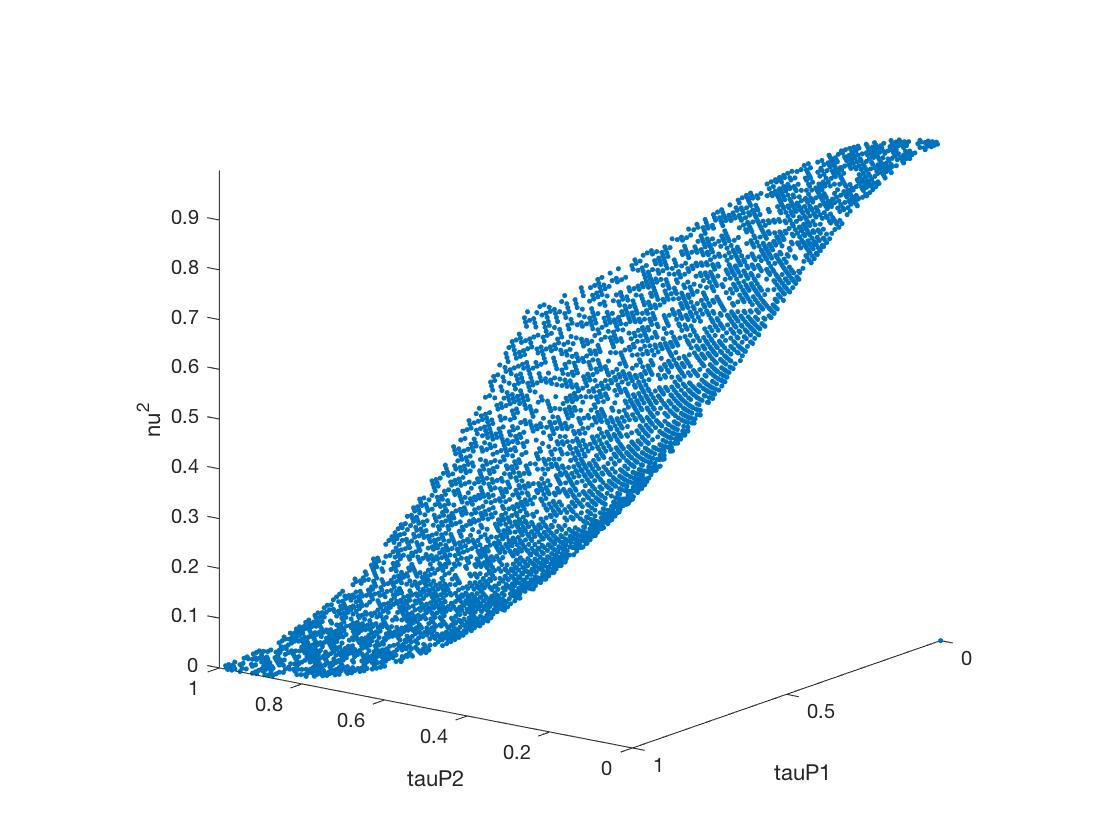
\includegraphics[width=9cm]{images/filter1e.jpg}
  \caption{Численное приближение в MATLAB}
  \label{fig:sub1}
\end{subfigure}%
\begin{subfigure}{.5\textwidth}
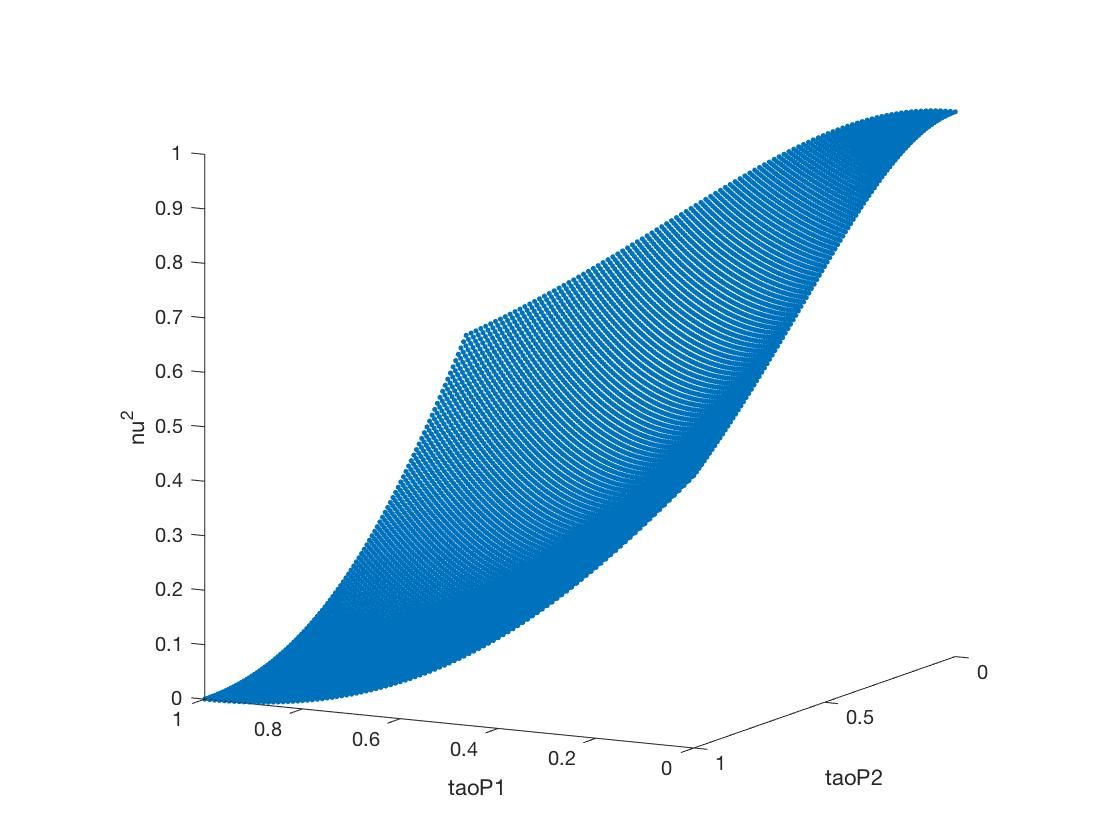
\includegraphics[width=9cm]{images/filter1_1.jpg}
  \caption{Вычисленный по \eqref{filter1_max}}
  \label{fig:sub2}
\end{subfigure}
\caption{График зависимости $\nu^2$ от $\tau_{p1}, \tau_{p2}$}
\label{fig:filter1_fig}
\end{figure}

\section{Оценка области захвата для систем ФАПЧ с фильтром $\frac{(1+\tau_{z1}x)^2}{(1+\tau_{p1}x)^2}$}
 Рассмотрим передаточную функцию:
 \begin{equation}\label{filter2}
 \begin{aligned}
K(x) = \frac{(1+\tau_{z1}x)^2}{(1+\tau_{p1}x)^2}
 \end{aligned}
\end{equation}
Предположим, что нелинейность $f(\sigma)=\phi(\sigma)$ имеет изолированные нули и удовлетворяет ???????.
Неравенство $\tau_{z1} \neq \tau_{p1}$ гарантирует, что функция $\chi(p) = x^{-1}K(x)$ не приводима. Тогда по теореме ???? пара $(A,B)$ управляема. Заметим
 \begin{equation}
 \begin{aligned}
\text{det}(xI-A) = x^2 + 2\tau_{z1}^{-1}x + \tau_{z1}^{-2}
 \end{aligned}
\end{equation}
матрица $A$ - матрица Гурвица. Найдем $\varepsilon, \delta, \varkappa, \tau$ так, что бы максимизировать $\nu$. Для этого подставим \eqref{filter2} в условие теоремы \ref{th1} и перенесем все в левую часть неравенства. В результате преобразований первое условие теоремы \ref{th1} принимает следующий вид:
 \begin{equation}\label{second_condition}
 \begin{aligned}
&\tau_{p1}^4\tau t^3 +(- \tau_{z1}^4\varepsilon - \tau_{z1}^4\tau + 2\tau_{p1}^2\tau- \tau_{p1}^4\delta + \tau_{z1}^2\tau_{p1}^2\varkappa)t^2  +\\
&+( \tau- \tau_{z1}^2\varkappa - 2\tau_{z1}^2\varepsilon - \tau_{p1}^2\varkappa- 2\tau_{z1}^2\tau+ 4\tau_{z1}b\varkappa- 2\tau_{p1}^2\delta)t + (\varkappa-\varepsilon - \tau - \delta)  \geq 0\\
&t = x^2 \geq 0
 \end{aligned}
\end{equation}
\subsection{$\tau = 0$}
Положим в \eqref{second_condition} $\tau = 0$, тогда первое условие теоремы принимает следующий вид:
 \begin{equation}\label{second_condition_tau_zero}
 \begin{aligned}
&(\tau_{z1}^2\tau_{p1}^2\varkappa - \tau_{z1}^4\varepsilon - \tau_{p1}^4\delta)t^2 +( 4\tau_{z1}\tau_{p1}\varkappa - \tau_{z1}^2\varkappa - 2\tau_{z1}^2\varepsilon - \tau_{p1}^2\varkappa - 2\tau_{p1}^2\delta)t + (\varkappa-\varepsilon - \delta)  \geq 0\\
&t = x^2 \geq 0
 \end{aligned}
\end{equation}
Обозначим:
 \begin{equation}
 \begin{aligned}
&A = \tau_{z1}^2\tau_{p1}^2\varkappa - \tau_{z1}^4\varepsilon - \tau_{p1}^4\delta\\
&B = 4\tau_{z1}\tau_{p1}\varkappa - \tau_{z1}^2\varkappa - 2\tau_{z1}^2\varepsilon - \tau_{p1}^2\varkappa - 2\tau_{p1}^2\delta\\
&C = \varkappa-\varepsilon - \delta
 \end{aligned}
\end{equation}
Для того, что бы выполнялось \eqref{second_condition_tau_zero} нужно потребовать: $A \geq 0$ и $C \geq 0$, тогда  при $B \geq 0$, тогда уравнение не имеет положительных корней, т.е. выполняется \eqref{second_condition_tau_zero}. Не умаляя общности можем считать $\varkappa = 1$. Получили задачу нахождения условного экстремума при условии:
 \begin{equation}\label{filter2_1_area}
 \begin{aligned}
&\tau_{z1}^2\tau_{p1}^2 - \tau_{z1}^4\varepsilon - \tau_{p1}^4\delta \geq 0\\
&4\tau_{z1}\tau_{p1} - \tau_{z1}^2 - 2\tau_{z1}^2\varepsilon - \tau_{p1}^2 - 2\tau_{p1}^2\delta \geq 0\\
&1-\varepsilon - \delta \geq 0
 \end{aligned}
\end{equation}
Максимум может достигаться на границе, или в точках понижения ранга. Представим $\varepsilon$ как $\varepsilon(\delta)$ и рассмотрим функцию $\varepsilon\delta$ на границе области \eqref{filter2_1_area}
 \begin{equation}\label{filter2_1_area_border}
 \begin{aligned}
&\frac{\tau_{p1}^2}{\tau_{z1}^2} - \frac{\tau_{p1}^4}{\tau_{z1}^4}\delta =\varepsilon\\
&2\frac{\tau_{p1}}{\tau_{z1}} - \frac{1}{2} - \frac{\tau_{p1}^2}{2\tau_{z1}^2} - \frac{\tau_{p1}^2}{\tau_{z1}^2}\delta =  \varepsilon\\
&\varepsilon = 1 - \delta
 \end{aligned}
\end{equation}
 Для этого найдем пересечения прямых \eqref{filter2_1_area_border}:
  \begin{equation}
 \begin{aligned}
&\delta = \frac{1}{1+z^2}, \varepsilon = \frac{z^2}{1+z^2}\\
&\delta = \frac{1-q}{1-z^2}, \varepsilon = \frac{q-z^2}{1-z^2}\\
&\delta = \frac{z^2-q}{z^4-z^2}, \varepsilon = z^2 - \frac{z^4(z^2-q)}{z^4-z^2}\\
&z = \frac{\tau_{p1}}{\tau_{z1}}\\
&q = 2z - \frac{1}{2} - \frac{1}{2}z^2\\
 \end{aligned}
\end{equation}
Оценки максимума на границе \eqref{filter2_1_area_border}:
  \begin{equation}
 \begin{aligned}
&\delta = \frac{1}{2}, \varepsilon = \frac{1}{2}, \varepsilon\delta = \frac{1}{4}\\
&\delta = \frac{1}{2z^2}, \varepsilon = \frac{z^2}{2}, \varepsilon\delta = \frac{1}{4}\\
&\delta = \frac{q}{2z^2}, \varepsilon = \frac{q}{2}, \varepsilon\delta = \frac{q^2}{4z^2}\\
 \end{aligned}
\end{equation}
  Максимум функции $\nu^2 = \frac{4\varepsilon\delta}{\varkappa^2}$ представлен на графике.

При $B < 0$ по теореме Декарта уравнение может иметь 2 корня. В этой ситуации потребуем отрицательность дискриминанта:
 \begin{equation}
 \begin{aligned}
&-4\tau_{z1}^4 \varepsilon \delta + 8\tau_{z1}^4 \varepsilon + \tau_{z1}^4 - 16\tau_{z1}^3 \tau_{p1} \varepsilon - 8\tau_{z1}^3 \tau_{p1} + 8\tau_{z1}^2 \tau_{p1}^2 \varepsilon \delta + 8\tau_{z1}^2 \tau_{p1}^2 \varepsilon + 8\tau_{z1}^2 \tau_{p1}^2 \delta + \\
& + 14\tau_{z1}^2 \tau_{p1}^2 - 16\tau_{z1} \tau_{p1}^3 \delta - 8\tau_{z1} \tau_{p1}^3 - 4\tau_{p1}^4 \varepsilon \delta + 8\tau_{p1}^4 \delta + \tau_{p1}^4 \leq 0
 \end{aligned}
\end{equation}

 \begin{equation}
 \begin{aligned}
4(\tau_{z1}^2-\tau_{p1}^2)^2(2\varepsilon\tau_{z1}^2-\varepsilon\delta+2\delta\tau_{p1}^2)+(\tau_{z1}-\tau_{p1})^2(\tau_{z1}^2-6\tau_{z1}\tau_{p1}+\tau_{p1}^2)\leq 0
 \end{aligned}
\end{equation}

 \begin{equation}
 \begin{aligned}
4(\tau_{z1}+\tau_{p1})^2(2\varepsilon\tau_{z1}^2-\varepsilon\delta+2\delta\tau_{p1}^2)+(\tau_{z1}^2-6\tau_{z1}\tau_{p1}+\tau_{p1}^2)\leq 0
 \end{aligned}
\end{equation}

  \begin{equation}
 \begin{aligned}
a\varepsilon + b\delta \geq \varepsilon\delta
 \end{aligned}
\end{equation}

\subsection{$\tau > 0$}
Предположим в \eqref{second_condition} $\tau > 0$ и разделим на $\tau_{p1}^4\tau$. Не умаляя общности, можем считать $\tau = 1$, тогда \eqref{second_condition} принимает следующий вид:
 \begin{equation}
 \begin{aligned}
&t^3 +at^2 +bt + c  \geq 0\\
&A = \frac{1}{\tau_{p1}^4}(- \tau_{z1}^4\varepsilon - \tau_{z1}^4 + 2\tau_{p1}^2- \tau_{p1}^4\delta + \tau_{z1}^2\tau_{p1}^2\varkappa)\\
&B = \frac{1}{\tau_{p1}^4}( 1- \tau_{z1}^2\varkappa - 2\tau_{z1}^2\varepsilon - \tau_{p1}^2\varkappa- 2\tau_{z1}^2+ 4\tau_{z1}\tau_{p1}\varkappa- 2\tau_{p1}^2\delta)\\
&C = \frac{1}{\tau_{p1}^4}(\varkappa-\varepsilon - 1 - \delta)\\
&t = x^2 \geq 0
 \end{aligned}
\end{equation}
Заметим, что по теореме Декарта: $a \geq 0, b \geq 0, c \geq 0$

\section{Оценка области захвата для систем ФАПЧ с фильтром $\frac{(1+\tau_{z1}x)(1+\tau_{z2}x)}{(1+\tau_{p1}x)(1+\tau_{p2}x)}$}
 Рассмотрим передаточную функцию:
 \begin{equation}\label{filter3}
 \begin{aligned}
K(x) = \frac{(1+\tau_{z1}x)(1+\tau_{z2}x)}{(1+\tau_{p1}x)(1+\tau_{p2}x)}
 \end{aligned}
\end{equation}
Представим \eqref{filter3} в виде:
 \begin{equation}\label{filter3-1}
 \begin{aligned}
&K(x) = \frac{1+\alpha_1\beta_1x + \alpha_2\beta_2x^2}{1+\alpha_1x + \alpha_2x^2}\\
&\alpha_1 = \tau_{p1} + \tau_{p2}\text{,}\quad 
\alpha_2 = \tau_{p1}\tau_{p2}\text{,}\quad 
\beta_1 = \frac{\tau_{z1}+\tau_{z2}}{\tau_{p1}+\tau_{p2}}\text{,}\quad 
\beta_2 = \frac{\tau_{z1}\tau_{z2}}{\tau_{p1}\tau_{p2}}
 \end{aligned}
\end{equation}
Предположим:
 \begin{equation}\label{restriction-1}
 \begin{aligned}
\beta_1 < \beta_2 < 1
 \end{aligned}
\end{equation}
Предположим, что нелинейность $f(\sigma)=\phi(\sigma)$ имеет изолированные нули и удовлетворяет ???????.
Неравенство \eqref{restriction-1} гарантирует, что функция $\chi(p) = x^{-1}K(x)$ не приводима. Тогда по теореме ???? пара $(A,B)$ управляема. Заметим
 \begin{equation}
 \begin{aligned}
\text{det}(xI-A) = x^2 + \alpha_1\alpha_2^{-1}x + \alpha_2^{-1}
 \end{aligned}
\end{equation}
матрица $A$ - матрица Гурвица. Найдем $\varepsilon, \delta, \varkappa, \tau$ так, что бы максимизировать $\nu$. Для этого подставим \eqref{filter3-1} в условие теоремы \ref{th1} и перенесем все в левую часть неравенства. В результате преобразований первое условие теоремы \ref{th1} принимает следующий вид:
 \begin{equation}
 \begin{aligned}
&\alpha_2^2\tau t^3 + (\alpha_1^2\tau - 2\alpha_2\tau - \alpha_2^2\delta - \alpha_2^2\beta_2^2\varepsilon - \alpha_2^2\beta_2^2\tau + \alpha_2^2\beta_2\varkappa)t^2 +\\
&+ (\tau - \alpha_2\varkappa + 2\alpha_2\delta - \alpha_1^2\delta - \alpha_1^2\beta_1^2\varepsilon - \alpha_1^2\beta_1^2\tau - \alpha_2\beta_2\varkappa + 2\alpha_2\beta_2\varepsilon + 2\alpha_2\beta_2\tau + \alpha_1^2\beta_1\varkappa)t + \\
&+ \varkappa - \varepsilon - \tau - \delta \geq 0
 \end{aligned}
\end{equation}
Положим $\tau = 0$:
 \begin{equation}
 \begin{aligned}
&(-\varepsilon\alpha_2^2\beta_2^2 + \varkappa\alpha_2^2\beta_2 - \delta\alpha_2^2)t^2 + (-\varepsilon\alpha_1^2\beta_1^2 + \varkappa\alpha_1^2\beta_1 - \delta\alpha_1^2 - \alpha_2\varkappa + 2\alpha_2\delta - \alpha_2\beta_2\varkappa + 2\alpha_2\beta_2\varepsilon)t +\\
& + \varkappa - \varepsilon - \delta \geq 0
 \end{aligned}
\end{equation}
Не умаляя общности можем считать $\varkappa = 1$:
 \begin{equation}
 \begin{aligned}
&(-\varepsilon\alpha_2^2\beta_2^2 + \alpha_2^2\beta_2 - \delta\alpha_2^2)t^2 + (-\varepsilon\alpha_1^2\beta_1^2 + \alpha_1^2\beta_1 - \delta\alpha_1^2 - \alpha_2 + 2\alpha_2\delta - \alpha_2\beta_2 + 2\alpha_2\beta_2\varepsilon)t +\\
& + 1 - \varepsilon - \delta \geq 0
 \end{aligned}
\end{equation}
Заметим, что $\varepsilon \leq 1 - \delta$. Для максимизации $\varepsilon\delta$ положим $\varepsilon = 1-\delta$.
 \begin{equation}
 \begin{aligned}
(\alpha_2^2\beta_2 - \alpha_2^2\delta - \alpha_2^2\beta_2^2 + \alpha_2^2\beta_2^2\delta)t + \alpha_2\beta_2 - \alpha_2 + 2\alpha_2\delta + \alpha_1^2\beta_1 - \alpha_1^2\delta - \alpha_1^2\beta_1^2 + \alpha_1^2\beta_1^2\delta - 2\alpha_2\beta_2\delta \geq 0
 \end{aligned}
\end{equation}
Нужно потребовать что бы выполнялось следущее условие
 \begin{equation}
 \begin{aligned}
\alpha_2\beta_2 - \alpha_2 + 2\alpha_2\delta + \alpha_1^2\beta_1 - \alpha_1^2\delta - \alpha_1^2\beta_1^2 + \alpha_1^2\beta_1^2\delta - 2\alpha_2\beta_2\delta \geq 0
 \end{aligned}
\end{equation}
Тогда
 \begin{equation}
 \begin{aligned}
&\alpha_2\beta_2 - \alpha_2 + 2\alpha_2\delta + \alpha_1^2(\beta_1 - \delta - \beta_1^2 + \beta_1^2\delta) - 2\alpha_2\beta_2\delta \geq 0 \\
&\alpha_1^2 \geq \frac{\alpha_2(1-\beta_2) - 2\alpha_2\delta(1-\beta_2)}{\beta_1(1-\beta_1) - \delta + \beta_1^2\delta} > \frac{\alpha_2(1-\beta_2)}{\beta_1(1-\beta_1) - \delta + \beta_1^2\delta} \xrightarrow[\delta \rightarrow 0]{} \frac{\alpha_2(1-\beta_2)}{\beta_1(1-\beta_1)}
 \end{aligned}
\end{equation}
Получили
 \begin{equation}
 \begin{aligned}
\alpha_1^2 > \frac{\alpha_2(1-\beta_2)}{\beta_1(1-\beta_1)}
 \end{aligned}
\end{equation}
Так как максимальное значение достигается на границе положим 
 \begin{equation}
 \begin{aligned}
\alpha_2\beta_2 - \alpha_2 + 2\alpha_2\delta + \alpha_1^2\beta_1 - \alpha_1^2\delta - \alpha_1^2\beta_1^2 + \alpha_1^2\beta_1^2\delta - 2\alpha_2\beta_2\delta = 0
 \end{aligned}
\end{equation}
Тогда 
 \begin{equation}
 \begin{aligned}
\delta = \frac{\alpha_1^2(1-\beta_1)\beta_1 - \alpha_2(1-\beta_2)}{\alpha_1^2(1-\beta_1^2) - 2\alpha_2(1-\beta_2)}
 \end{aligned}
 \end{equation}
Получили, что
 \begin{equation}
 \begin{aligned}
\nu^2 < 4\frac{[\alpha_1^2(1-\beta_1) - \alpha_2(1-\beta_2)][\alpha_1^2(1-\beta_1)\beta_1 - \alpha_2(1-\beta_2)]}{[\alpha_1^2(1-\beta_1^2) - 2\alpha_2(1-\beta_2)]^2}
 \end{aligned}
 \end{equation}
\end{document}  
% КОНЕЦ ДОКУМЕНТА !